\section{ARMA and ARMAX models}

Consider the ARMA and ARMAX class of models:
\[\mathcal{M}(\vartheta): y(t)=\dfrac{B(z)}{A(z)}u(t-d)+\dfrac{C(z)}{A(z)}e(t)\qquad e(t \sim WN(0,\lambda^2))\]
Here, we have:
\[\begin{cases}
    A(z)=1-a_1z^{-1}-a_zz^{-2}-\dots-a_mz^{-m} \\
    B(z)=b_1+b_2z^{-1}+b_3z^{-2}+\dots+b_pz^{-p+1} \\
    C(z)=1+c_1z^{-1}+c_2z^{-2}+\dots-c_nz^{-n}
\end{cases}\]
Where: 
\[\vartheta=\begin{bmatrix}
    a_1 & \dots & a_m & b_1 & \dots & b_p & c_1 & \dots & c_n
\end{bmatrix}^T\]

We begin by determining the predictor using the long division between $C(z)$ and $A(z)$. 
Both transfer functions are monic since they are in canonical form. 
Consequently, the division between the two yields unity after a single step. 
Thus, we have $E(z)=1$ and $z^{-k}F(z)=C(z)-A(z)$.

From this outcome, we derive the one-step ahead predictor as:

The one-step ahead prediction error associated with this predictor equals:
\[\hat{y}(t\mid t-1)=\dfrac{F(z)}{C(z)}z^{-1}y(t)+\dfrac{B(z)}{C(z)}u(t-d)=\dfrac{C(z)-A(z)}{C(z)}y(t)+\dfrac{B(z)}{C(z)}u(t-d)\]
The one-step ahead prediction error associated with this predictor can be expressed as:
\begin{align*}
    \varepsilon(t\mid t-1,\vartheta)&=y(t)-\hat{y}(t\mid t-1,\vartheta)=y(t)-\dfrac{C(z)-A(z)}{C(z)}y(t)-\dfrac{B(z)}{C(z)}u(t-d)\\
                                &=y(t)\left(1-\dfrac{C(z)A(z)}{C(z)}\right) - \dfrac{B(z)}{C(z)}u(t-d) \\
                                &=\dfrac{A(z)}{C(z)}y(t)-\dfrac{B(z)}{C(z)}u(t-d)
\end{align*}
The cost function related to this predictor then becomes:
\[J_N(\vartheta)=\dfrac{1}{N}\sum_{t=1}^N \varepsilon(t\mid t-1,\vartheta)^2\]
This function is no longer quadratic in $\vartheta$, necessitating the handling of a nonlinear optimization problem.
To address this problem, we employ an iterative approach:
\begin{enumerate}
    \item Initialize the algorithm with an initial estimate $\vartheta_1$ randomly chosen.
    \item Define an update rule $\vartheta^{i+1}=f\left(\vartheta^{i}\right)$.
    \item The sequence of estimates should converge to $\hat{\vartheta}_N$.
\end{enumerate}
However, there are challenges with this procedure, notably the selection of an update rule ensuring convergence and finding appropriate initialization values.

\subsection{Initialization}
We have two main approaches for initialization:
\begin{itemize}
    \item \textit{Iterative algorithms}: these algorithms are guaranteed to converge to a minimum, albeit potentially a local one.
    \item \textit{Multiple initializations} (empirical approach): here, we start the problem with multiple random guesses and apply the update rule to each. 
        Eventually, we obtain several results, from which we select the solution with the minimum value of $J_N(\vartheta)$. 
        While this method increases the chance of finding the best result, it also escalates computational costs, especially with a higher number of attempts.
\end{itemize}

\subsection{Update rule}
The most commonly used update rule is Newton's method. 
Let $V^i(\vartheta)$ denote the second-order Taylor expansion of $J_N(\vartheta)$ in the vicinity of $\vartheta^i$:
\[V^{i}(\vartheta)=J_N(\vartheta^i)+(\vartheta-\vartheta^i)\dfrac{\partial J_N(\vartheta)}{\partial\vartheta}+\dfrac{1}{2}(\vartheta-\vartheta^i)^T\dfrac{\partial^2 J_N(\vartheta)}{\partial\vartheta^2}(\vartheta-\vartheta^i)\]
This is evaluated at $\vartheta=\vartheta^i$. 
To locate the minimum of this curve, we set the first derivative equal to zero:
\[\dfrac{\partial V^i(\vartheta)}{\partial\vartheta}=0\]
This is done at $\vartheta=\vartheta^{i+1}$. 
Consequently, we have:
\[\dfrac{\partial V^i(\vartheta)}{\partial\vartheta}=\dfrac{\partial J_N(\vartheta)}{\partial\vartheta}+\dfrac{\partial^2 J_N(\vartheta)}{\partial\vartheta^2}(\vartheta-\vartheta^i)=0\]
This is evaluated at $\vartheta=\vartheta^{i+1}$. 
Ultimately, we obtain:
\[\vartheta^{i+1}=\vartheta^i-\left[ \dfrac{\partial^2 J_N(\vartheta)}{\partial\vartheta^2} \right]^{-1}\dfrac{\partial J_N(\vartheta)}{\partial\vartheta}\]
This is evaluated at $\vartheta=\vartheta^{i}$.

\paragraph*{Gradient}       
Let's compute the gradient of the cost function:
\[\dfrac{\partial J_N(\vartheta)}{\partial\vartheta} =\dfrac{d}{d\vartheta}\left[ \dfrac{1}{N}\sum_{t=1}^{N} \varepsilon(t,\vartheta)^2 \right]=\left[ \dfrac{1}{N}\sum_{t=1}^{N} \dfrac{d}{d\vartheta}\varepsilon(t,\vartheta)^2 \right]=\dfrac{2}{N}\sum_{t=1}^{N}\varepsilon(t,\vartheta)\dfrac{d\varepsilon(t,\vartheta)}{d\vartheta}\]
Now, let's compute the second-order gradient of the cost function:
\begin{align*}
    \dfrac{\partial^2 J_N(\vartheta)}{\partial\vartheta^2}  &=\dfrac{d}{d\vartheta}\left[ \dfrac{2}{N}\sum_{t=1}^{N}\varepsilon(t,\vartheta)\dfrac{d\varepsilon(t,\vartheta)}{d\vartheta} \right] \\
                                                            &=\dfrac{2}{N}\sum_{t=1}^{N}\dfrac{d\varepsilon(t,\vartheta)}{d\vartheta}\left(\dfrac{d\varepsilon(t,\vartheta)}{d\vartheta}\right)^T + \underbrace{\dfrac{2}{N}\sum_{t=1}^{N}\varepsilon(t,\vartheta)\left(\dfrac{d\varepsilon(t,\vartheta)}{d\vartheta}\right)}_{\text{negligible}}  \\
                                                            &=\dfrac{2}{N}\sum_{t=1}^{N}\dfrac{d\varepsilon(t,\vartheta)}{d\vartheta}\left(\dfrac{d\varepsilon(t,\vartheta)}{d\vartheta}\right)^T
\end{align*}
The second part is negligible because the value of $\varepsilon(\vartheta)$ is small. 
By considering only the first part, the estimate of the Hessian will always be non-negative, ensuring convergence.

\paragraph*{Final update rule}
After all considerations, the final version of the update rule is:
\[\vartheta^{i+1}=\vartheta^i-\left[ \dfrac{2}{N}\sum_{t=1}^{N}\dfrac{d\varepsilon(t,\vartheta)}{d\vartheta}\left(\dfrac{d\varepsilon(t,\vartheta)}{d\vartheta}\right)^T \right]^{-1}\left[\dfrac{2}{N}\sum_{t=1}^{N}\varepsilon(t,\vartheta)\dfrac{d\varepsilon(t,\vartheta)}{d\vartheta}\right]\]
This is evaluated at $\vartheta^i$.

\paragraph*{Estimation error}
The estimation error $\varepsilon(t,\vartheta)$ is given by:
\begin{align*}
    \varepsilon(t,\vartheta)    &=\dfrac{A(z)}{C(z)}y(t)-\dfrac{B(z)}{C(z)}u(t-d) \\
                                &=\dfrac{1+a_1z^{-1}+\dots+a_mz^{-m}}{1+c_1z^{-1}+c_2z^{-2}+\dots-c_nz^{-n}}y(t)-\dfrac{b_1+b_2z^{-1}+b_3z^{-2}+\dots+b_pz^{-p+1}}{1+c_1z^{-1}+c_2z^{-2}+\dots-c_nz^{-n}}u(t-d)
\end{align*}
We need to compute the derivative with respect to all elements of the vector: 
\[\vartheta=\begin{bmatrix}
    a_1 & \dots & a_m & b_1 & \dots & b_p & c_1 & \dots & c_n
\end{bmatrix}^T\]

\paragraph*{Parameters of $A(z)$}
Let's begin by considering the parameter $a_1$:
\begin{align*}
    \dfrac{\partial\varepsilon(t,\vartheta)}{\partial a_1}  &=\dfrac{\partial}{\partial a_1}\left[ \dfrac{1+a_1z^{-1}+\dots+a_mz^{-m}}{1+c_1z^{-1}+c_2z^{-2}+\dots-c_nz^{-n}}y(t)\right] - \underbrace{\dfrac{\partial}{\partial a_1}\left[\dfrac{B(z)}{C(z)}u(t-d)\right]}_0 \\        
                                                            &=\dfrac{z^{-1}y(t)}{C(z)} \\
                                                            &=\dfrac{1}{C(z)}y(t-1)
\end{align*}
Let's define a signal $\alpha(t)=\frac{1}{C(z)}y(t)$, obtaining:
\[\dfrac{\partial\varepsilon(t,\vartheta)}{\partial a_1}=\alpha(t-1)\]
If we perform the same operation for all the $a_i$ in $\vartheta$, we obtain:
\[\begin{cases}
    \frac{\partial\varepsilon(t,\vartheta)}{\partial a_1}=\alpha(t-1) \\
    \frac{\partial\varepsilon(t,\vartheta)}{\partial a_2}=\alpha(t-2) \\
    \vdots \\
    \frac{\partial\varepsilon(t,\vartheta)}{\partial a_m}=\alpha(t-m)
\end{cases}\]

\paragraph*{Parameters of $B(z)$}
Let's begin by considering the parameter $b_1$:
\begin{align*}
    \dfrac{\partial\varepsilon(t,\vartheta)}{\partial b_1}  &=\underbrace{\dfrac{\partial}{\partial b_1}\left[ \dfrac{A(z)}{C(z)}y(t)\right]}_0 - \dfrac{\partial}{\partial a_1}\left[\dfrac{b_1+b_2z^{-1}+b_3z^{-2}+\dots+b_pz^{-p+1}}{1+c_1z^{-1}+c_2z^{-2}+\dots-c_nz^{-n}}u(t-d)\right] \\        
                                                            &=-\dfrac{1}{C(z)}u(t-d)
\end{align*}
Let's define a signal $\beta(t)=-\frac{1}{C(z)}u(t)$, obtaining: 
\[\dfrac{\partial\varepsilon(t,\vartheta)}{\partial b_1}=\beta(t-d)\]
If we perform the same operation for all the $b_i$ in $\vartheta$, we obtain:
\[\begin{cases}
    \frac{\partial\varepsilon(t,\vartheta)}{\partial b_1}=\beta(t-d) \\
    \frac{\partial\varepsilon(t,\vartheta)}{\partial b_2}=\beta(t-d-1) \\
    \vdots \\
    \frac{\partial\varepsilon(t,\vartheta)}{\partial a_p}=\beta(t-d-p+1)
\end{cases}\]

\paragraph*{Parameters of $C(z)$}
Considering the equation:
\[\varepsilon(t)=\dfrac{A(z)}{C(z)}y(t)-\dfrac{B(z)}{C(z)}u(t-d)\]
This can be rewritten as: 
\[C(z)\varepsilon(t)=A(z)y(t)-B(z)u(t-d)\]

Let's start by considering the parameter $c_1$:
\begin{align*}
    &\dfrac{d}{d c_1}\left[ C(z)\varepsilon(t) \right]=\dfrac{d}{dc_1}\left[ A(z)y(t)-B(z)u(t-d) \right] \rightarrow \\
    &\dfrac{dC(z)}{d c_1}\varepsilon(t) + \dfrac{d\varepsilon(t)}{d c_1}C(z)= 0 \rightarrow \\
    &z^{-1}\varepsilon(t)+C(z)\dfrac{\partial\varepsilon(t)}{\partial c_1} = 0 \rightarrow \\
    &\dfrac{\partial\varepsilon(t)}{\partial c_1}=-\dfrac{z^{-1}\varepsilon(t)}{C(z)}
\end{align*}
Let's define a signal $\gamma(t)=-\frac{1}{C(z)}\varepsilon(t)$, obtaining:
\[\dfrac{\partial\varepsilon(t,\vartheta)}{\partial c_1}=\gamma(t-1)\]
If we perform the same operation for all the $c_i$ in $\vartheta$, we obtain:
\[\begin{cases}
    \frac{\partial\varepsilon(t,\vartheta)}{\partial c_1}=\gamma(t-1) \\
    \frac{\partial\varepsilon(t,\vartheta)}{\partial c_2}=\gamma(t-2) \\
    \vdots \\
    \frac{\partial\varepsilon(t,\vartheta)}{\partial c_m}=\gamma(t-m)
\end{cases}\]

The block diagram for this method is as follows:
\begin{figure}[H]
    \centering
    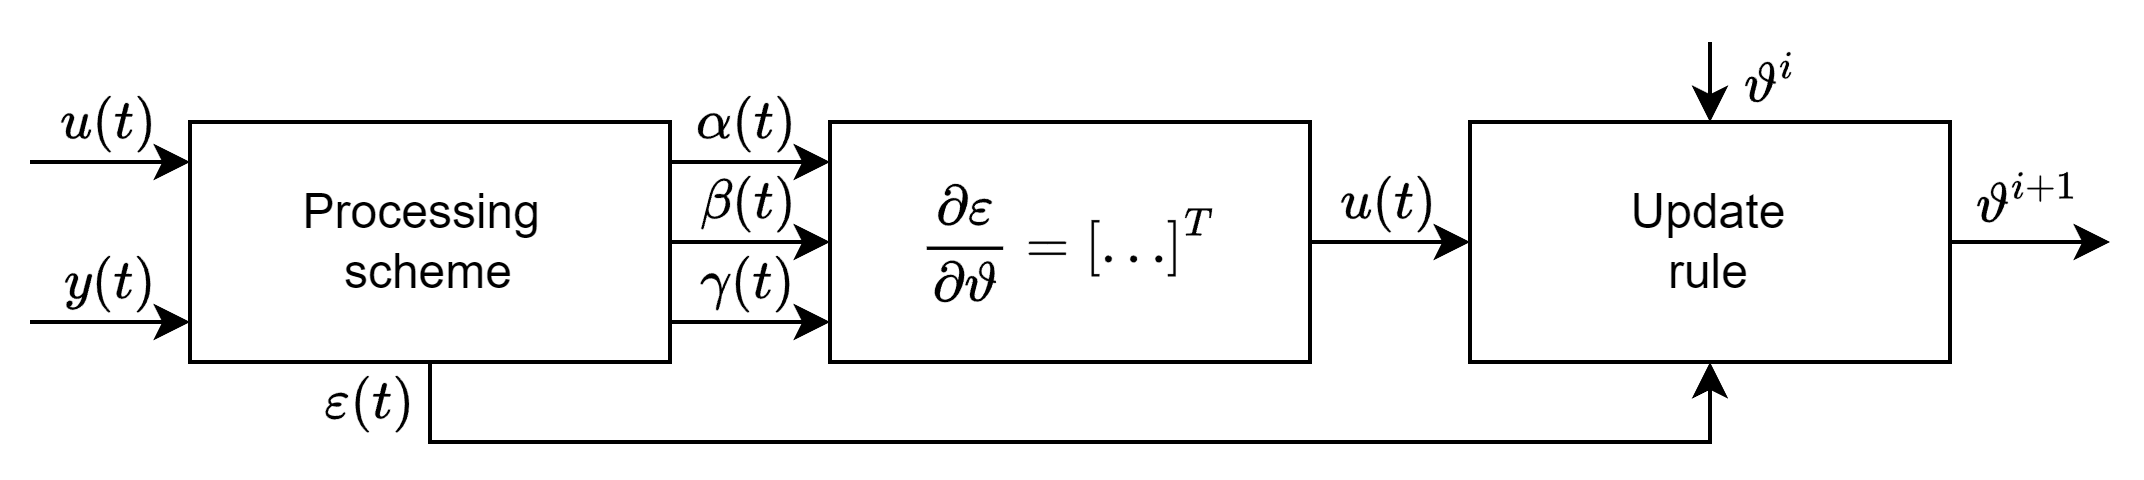
\includegraphics[width=0.75\linewidth]{images/iden.png}
    \caption{ARMAX identification procedure}
\end{figure}

In summary, the steps for the update rule are as follows:
\begin{enumerate}
    \item Compute polynomials $A(z,\vartheta^i)$, $B(z,\vartheta^i)$, and $C(z,\vartheta^i)$ at step $i$. 
    \item Compute the signals $\varepsilon(t, \vartheta^i)$, $\alpha(t, \vartheta^i)$, $\beta(t, \vartheta^i)$, and $\gamma(t, \vartheta^i)$. 
    \item Compute the gradient $\frac{\partial\varepsilon(t,\vartheta)}{\partial\vartheta}$.
    \item Update the parameter estimate: 
        \[\vartheta^{i+1}=\vartheta^i-\left[ \dfrac{2}{N}\sum_{t=1}^{N}\dfrac{d\varepsilon(t,\vartheta)}{d\vartheta}\left(\dfrac{d\varepsilon(t,\vartheta)}{d\vartheta}\right)^T \right]^{-1}\left[\dfrac{2}{N}\sum_{t=1}^{N}\varepsilon(t,\vartheta)\dfrac{d\varepsilon(t,\vartheta)}{d\vartheta}\right]\]
\end{enumerate}

After acquiring the inverse part via Quasi-Newton optimization, we strive for a balanced approach that prioritizes both robustness and accuracy during the estimation procedure. 
In instances where the estimate of the Hessian is numerically poorly conditioned, we employ:
\[\dfrac{\partial J_N(\vartheta)}{\partial\vartheta^2}=\dfrac{2}{N}\sum\dfrac{\partial\varepsilon(t,\vartheta)}{\partial\vartheta}\dfrac{\partial\varepsilon(t,\vartheta)}{\partial\vartheta}^T+\delta I\]
Here, $\delta$, referred to as the tuning parameter, needs to be kept sufficiently small to prevent significant fluctuations in the final outcome.